\documentclass[a4paper,12pt,titlepage]{scrartcl}
\usepackage[sc]{mathpazo} % Schrift - wie Funcky und in PDF zu Fonts beschrieben
\usepackage[T1]{fontenc}
\usepackage[utf8]{inputenc}
\usepackage[a-1b]{pdfx}
\usepackage[ngerman]{babel}
\usepackage[amssymb]{SIunits} 
\usepackage{graphicx} 
\usepackage{subfigure}                         
\usepackage{float}
\usepackage[iso,german]{isodate} %his package provides commands to switch between different date formats
\usepackage{hyperref}
\usepackage{listings}
\usepackage{graphicx}
\usepackage[export]{adjustbox}

\usepackage{fancyhdr}
\renewcommand{\headrulewidth}{0.5pt}
\renewcommand{\footrulewidth}{0.5pt}
%Abstand zwischen Absätzen, Zeilenabstände
\voffset26pt 
\parskip6pt
%\parindent1cm  %Rückt erste Zeile eines neuen Absatzes ein
\usepackage{setspace}
\onehalfspacing

\begin{document}
\pagenumbering{roman}
\titlehead
{
    \small
    {
        Technische Universität Ilmenau\\
        Fakulät IA\\
        Fachgebiet Biosignalverarbeitung\\

        Praktikum EKG-Signalanalyse\\
        WS 2021/22}
}

\title {Versuchsprotokoll}
\subtitle{EKG-Signalanalyse}
\author{}
\date{14. Januar 2022\\*[60pt]}

\title {Versuchsprotokoll: EKG-Signalanalyse}
\subtitle{Praktikumsbetreuer: Marc Heppner}
\author{Teilnehmer: Robert Jeutter \& Leonard Seifert}
\date{
    Datum Versuchsdurchführung: \quad 14.01.22\\
    Datum Protokollabgabe: \quad 28.01.22
}
\maketitle  %Erstellt das Titelblatt wie oben definiert

%Einstellungen zur Kopf- und Fußzeile
\pagestyle{fancy}
\fancyhead[R]{Praktikumsbericht: EKG-Signalanalyse}
\pagenumbering{arabic}
\newpage

% === Einverstaendniserklaerung ================================================
\vspace*{8cm}

Erklärung:

\noindent ,,Hiermit versichern wir, dass wir dieses Praktikum selbständig vorbereitet, mit dem Praktikumsleiter durchgeführt und selbständig nachbereitet haben und nur die angegebenen Quellen und Hilfsmittel verwendet haben.''

\newpage

\section{Vorbereitungsaufgaben}
\subsection{EKG-Vorverarbeitung}
\texttt{Entwickelung einer Strategie zur EKG-Vorverarbeitung. Bedenke dabei, dass die EKG-Vorverarbeitung maßgeblichen Einfluss auf die Qualität der QRS-\\ Detektion hat.}

Bei der EKG Signaldetektion enthält das auszuwertende Signal neben dem gewünschten EKG verschiedene Störsignale. Diese Störsignale können in zwei Kategorien eingeteilt werden: stochastische und deterministische Signale. In der Vorverarbeitung ist es unser Ziel die deterministischen Störungen zu entfernen.

Eines der bekannten niedrigfrequenten Signale entsteht durch die Atmung und bildet sich als Drift in dem Signal ab. Dieser Fehler kann mit einem Hochpass behoben werden, der die niederfrequenten Signale entfernt.

Desweiteren nutzen wir den bekannten Frequenzbereich in dem der größte Energieanteil des QRS Komplexes liegt zwischen 5-26 Hz mithilfe eines Bandpasses, um die Störsignale außerhalb dieses Bereiches im Vergleich zu unserem gewünschten Signal abzuschwächen.

Das Ergebnis der Vorverarbeitung soll ein driftarmes und von größeren deterministischen Störsignalen befreites Signal liefern.

\subsection{QRS-Detektion}
\texttt{Entwickelung einens Algorithmus zur adaptiven QRS-Detektion. 250 ms Zeit-\\vorlauf sollen dabei nicht überschritten werden}

\begin{enumerate}
    \item Hochpass zur Driftkompensation
          \begin{enumerate}
              \item Fourier Transformation
              \item entfernen niedriger Frequenzen
              \item Rücktransformation mit Inverser Fouriertransformation
          \end{enumerate}
    \item Bandpass zur Beschränkung auf niederfrequente Biosignale zwischen 5-26 Hz
    \item Minimale Distanz zwischen Peaks der R-Spitzen ermitteln
          \begin{enumerate}
              \item Kopie des Signal erstellen zur verlustfreien Bearbeitung
              \item Skalierung des Signals
              \item Kleine Peaks entfernen bzw. auf null setzten
              \item alle übrigen Peaks finden
              \item minimalen Abstand aller (übrigen) Peaks ermitteln
          \end{enumerate}
    \item Threshold festlegen (Halbe Signalstärke)
    \item Signalspitzen zwischen minimaler und maximaler Distanz, die über dem Threshold liegen, ermitteln
\end{enumerate}

\texttt{Entwickele zu diesem Algorithmus die zugehörige(n) MATLAB-Funktion(en)}

\begin{lstlisting}[basicstyle=\scriptsize, language=matlab]
function [R_Positionen, Entscheidungssignal, Schwellwertverlauf, Lernphase] 
= QRS_Detektion (EKG_Signal, fa);
    size = length(EKG_Signal); % Laenge des Signals
    % fourier transformation
    signal = fft(EKG_Signal);
    % entfernen niedriger freqzenzen anhand Laenge und Rate
    signal(1 : round(size*5/fa))=0;
    signal(end - round(size*5/fa) : end)=0;
    % inverse fourier transformation
    signal=real(ifft(signal));
    % bandpass fuer 5 bis 26 hz
    signal=bandpass(signal, [5 26], fa);

    % skalierung des Signals auf skala 1-10
    filtersignal=signal/(max(signal)/10);
    % entfernen aller peaks unterhalb des thresholds 10/2=5
    for data = 1:1:length(filtersignal)
        if filtersignal(data) < 5
            filtersignal(data) = 0;
        else
            filtersignal(data)=1;
        end
    end
    % finde alle uebrigen peaks, die ueber dem threshold lagen
    positions=find(filtersignal);
    % abstand der ersten beiden peaks
    distance=positions(2)-positions(1);
    % setzte den abstand auf das minimum zweier peaks in der reihe aller uebrigen peaks
    for data=1:1:length(positions)-1
        if positions(data+1)-positions(data)<distance
            distance=positions(data+1)-positions(data);
        end
    end

    % Mittel des Signals als Threshold
    avg = mean(signal) 
    
    % Absolute Peaks innerhalb des Zeitfensters finden
    [RPeaks, positions] = findpeaks(signal, 'MinPeakHeight', 1.5*avg, 
                    'MinPeakDistance', distance, "MaxPeakWidth", 250);
    R_Positionen = positions;
    Entscheidungssignal = signal;
    Schwellwertverlauf = RPeaks;
    Lernphase = 0; % Bedeutung nicht erklaert
end
\end{lstlisting}

Dieser Code ist derzeit nicht online fähig und passt sich keinen Signalstärkenänderungen an.

\newpage
\section{Praktikumsauswertung}
\subsection{EKG-Ableitung mit Hilfe des Biosignalverstärkers}
\texttt{Leiten Sie jeweils ein 5 minütiges EKG eines Studenten innerhalb der folgenden vier Phasen ab. Achten Sie dabei auf die Auswahl der Kanäle!
    \begin{itemize}
        \item Lagetyp-Phase: Proband liegt und atmet normal
        \item Ruhe-Phase: Proband liegt und atmet normal
        \item RESP-Phase: Proband liegt und atmet langsam tief ein und tief aus
        \item STEH-Phase: Proband steht und atmet normal
    \end{itemize}
}\vspace{1cm}

Diese Aufgabe entfiel, da das Praktikum über Webex stattfand. Die EKG Signale für weitere Aufgaben waren bereits in der Simulation vom Fachgebiet vorbereitet.

\newpage
\subsection{Bestimmung der elektrischen Herzachse}
\texttt{Mit Hilfe des Matlab-GUI „Datenanzeigen“ können die abgeleiteten Signale \\dargestellt und ausgewertet werden.}

\begin{figure}[ht]
    \begin{minipage}[t]{0.5\linewidth}
        \centering
        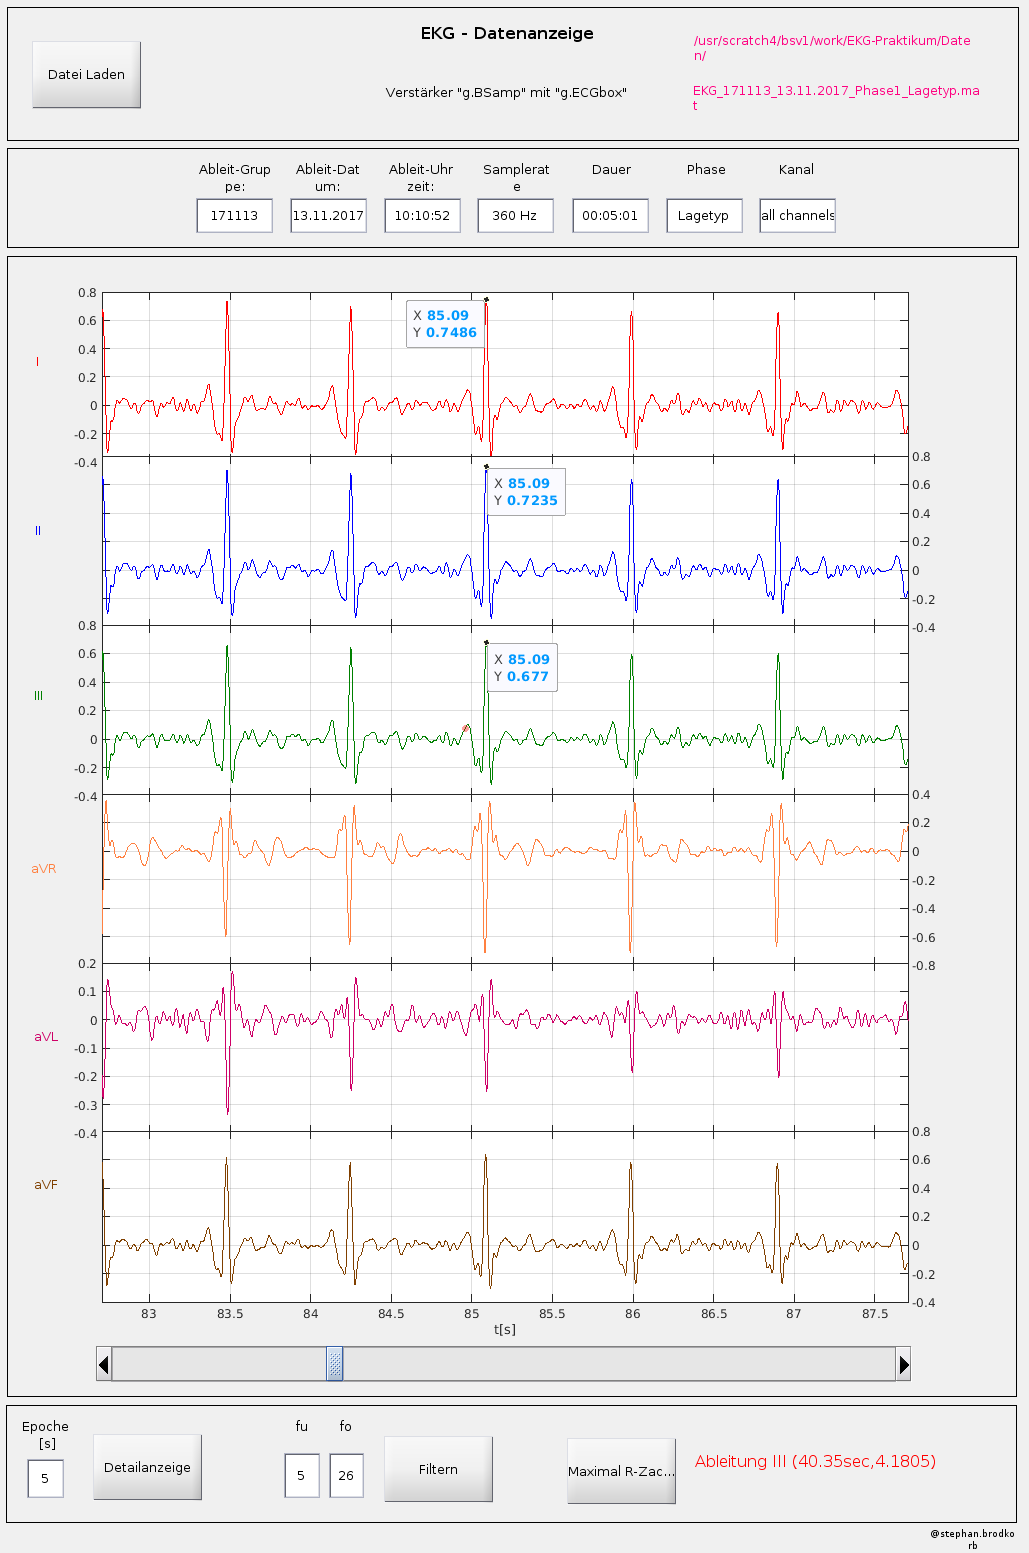
\includegraphics[width=0.9\linewidth, valign=t]{Assets/LaborBMT-15-11-03.png}
        \caption{Phase1\_Lagetyp.mat}
        \label{lagetyp}
    \end{minipage}%
    \begin{minipage}[t]{0.5\linewidth}
        Der vorgegebene Testdatensatz ,,Phase1\_Lagetyp.mat'' wurde in das Programm geladen. Das Signal wurde in der GUI mit einer unteren Filtergrenze von 5 Hz und oberen Filtergrenze von 26 Hz gefiltert.

        Für die Herzachsenbestimmung sollte kein Abschnitt zu Beginn des Messvorgangs verwendet werden, da dort oft Einschaltfehler der Messgeräte auftreten und der Patient unruhiger ist. Wir entschieden uns für die Epoche zwischen 83 und 87 Sekunden, da dieser Artefaktfrei ist (hier links in Abbildung \ref{lagetyp} zu sehen).

        Die höchste R-Zacke in dieser Epoche haben wir bei 85,09 Sekunden gemessen.
        Die Amplitude wurde mit den GUI ,,Data-Cursor'' ausgelesen. Diese sind für
        \begin{itemize}
            \item Kanal I: 0,7486 mV
            \item Kanal II: 0,7235 mV
            \item Kanal III: 0,677
        \end{itemize}
    \end{minipage}
\end{figure}

Die Funktionswerte werden in den, aus der Praktikumsanleitung vorgefertigten, Cabrera-Kreis eingetragen um den Lagetyp zu bestimmen.
Zur Umrechnung von mV in cm wenden wir den Maßstab [1mV:2cm] an. Aus der Vektoraddition der Schnittpunkte zweier Kanäle lässt sich die Herzachse in Grad messen.
Die Lagetypbestimmung ist in Abbildung \ref{Lagetypbestimmung} zu sehen.

Da wir mit einem anonymen Datensatz ohne bekanntes Alter des Probanden arbeiten, rechnen wir am ehesten mit dem durchschnittlichen Normaltyp. Diesen erhalten wir, eine weitere Diskussion entfällt dadurch.

\begin{figure}[h]
    \caption{Lagetypbestimmung mit Cabrera-Kreis}
    \label{Lagetypbestimmung}
    \centering
    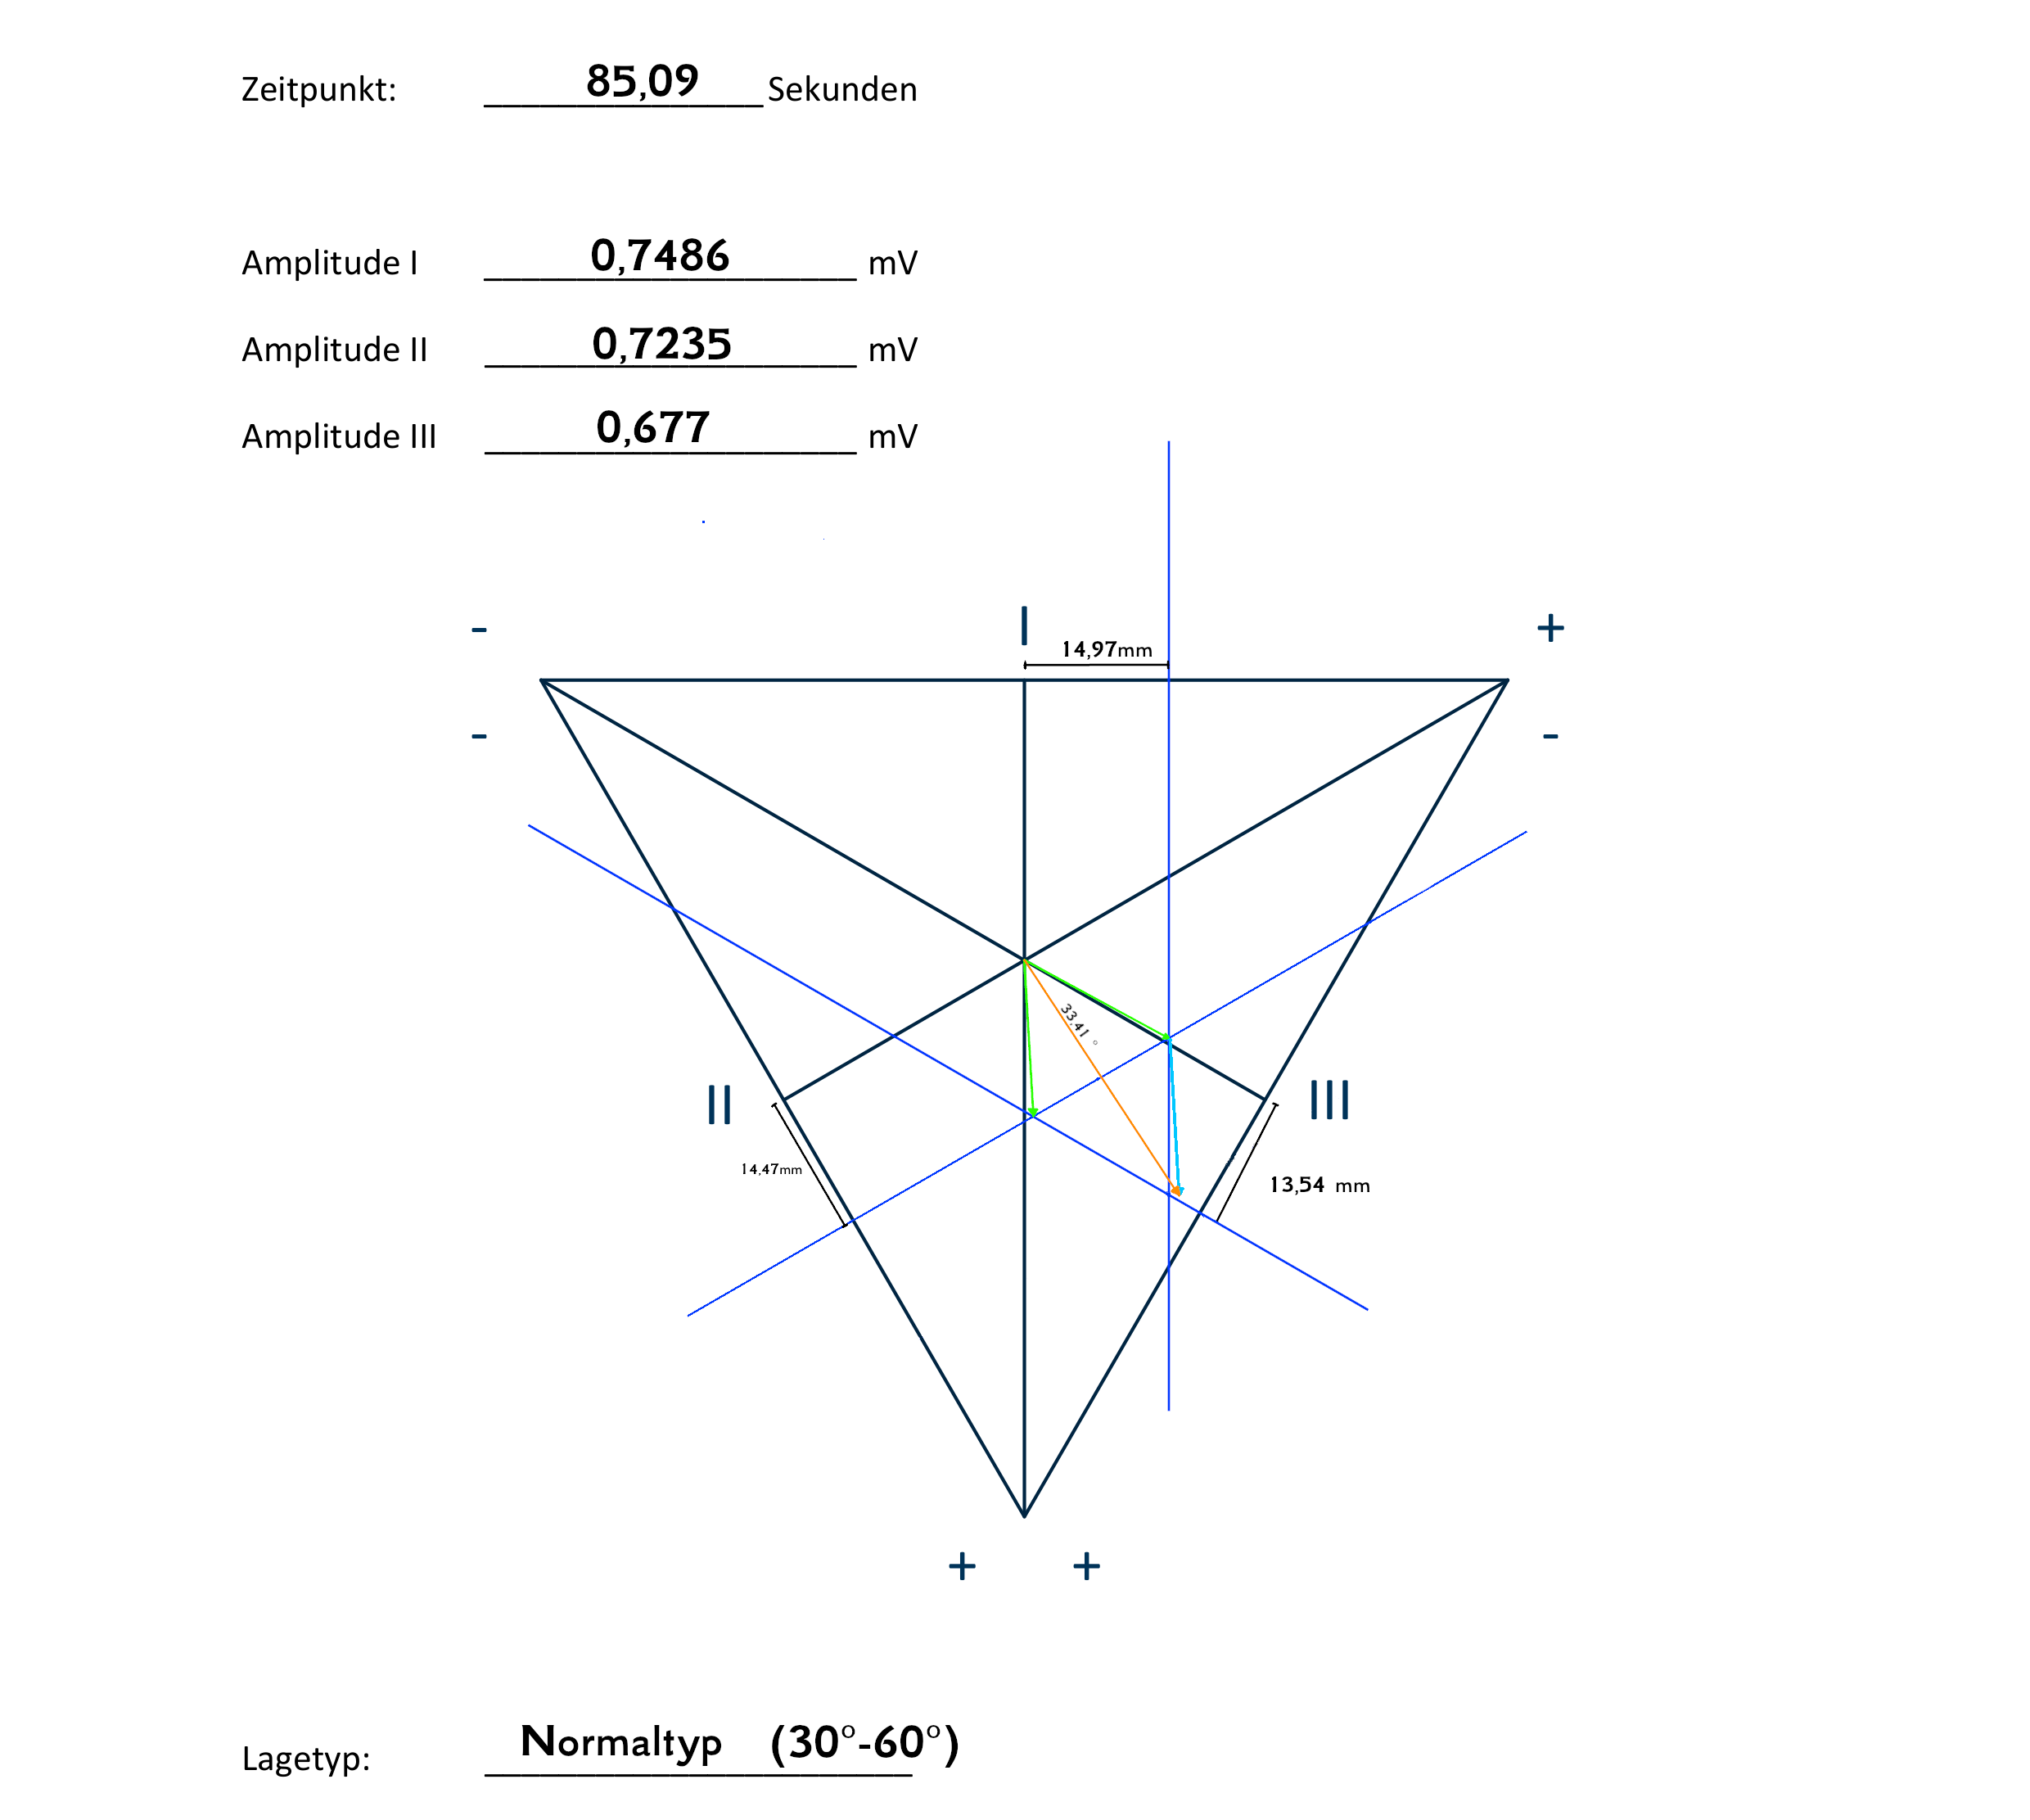
\includegraphics[width=\linewidth]{Assets/LaborBMT-Lagetyps.png}
\end{figure}


\cleardoublepage
\subsection{EKG-Vorverarbeitung}\label{EKG-Vorverarbeitung}
\texttt{Überprüfe die Wirksamkeit der vorgeschlagenen Vorverarbeitungsmethoden und deren Parametereinstellungen anhand der EKG-Signale der MIT-Datenbank.\\ Überlagere die Signale mit einem Drift und einer 50 Hz-Sinusschwingung!}

In der Ansicht zur EKG Vorverarbeitung zeigt die GUI vier Kanäle. Kanal ,,Rohsignal'' zeigt das Eingangssignal ohne Fehler. Kanal 1 zeigt das Rohsignal nach Überlagerung mit einem Drift und einer 50Hz Störungs-Schwingung. Kanäle 2 und 3 werden für die Vorverarbeitungsansicht verwendet, durch Anwenden von Filtern können die Signalausgaben hier gezeigt werden.

\begin{figure}[ht]
    \begin{minipage}[t]{0.5\linewidth}
        \centering
        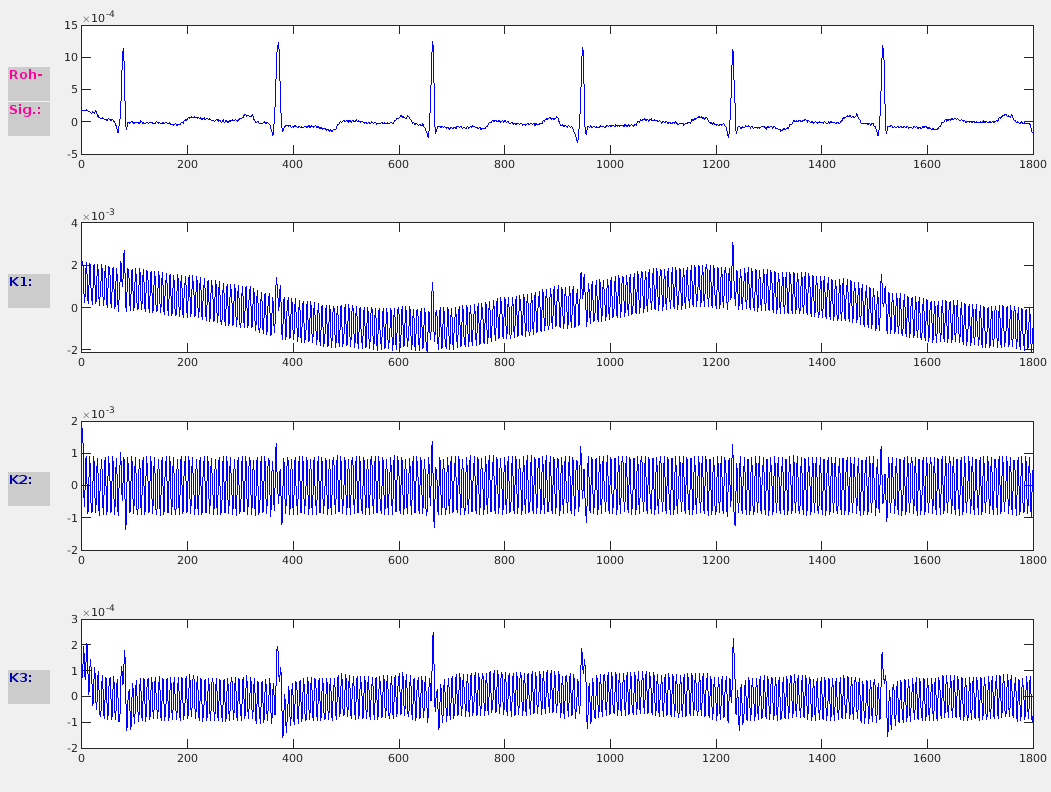
\includegraphics[width=0.9\linewidth, valign=t]{Assets/LaborBMT-15-20-37.png}
        \caption{DB100 V1}
        \label{db100v1}
    \end{minipage}%
    \begin{minipage}[t]{0.5\linewidth}
        Mit Datenbank 100 wird das EKG Signal geladen und in Kanal ,,Rohsignal'' dargestellt. Für die erste Vorverarbeitung wurde ein Hochpass 1. Ordnung mit $fa=360$ und $fo=25$ des Types IIR-Einseitig Butterworth angewendet und in Kanal ,,K2'' abgebildet. Dadurch wurde der Drift entfernt, Rauschen ist noch vorhanden, Signalspitzen wurden verzerrt.

        Kanal ,,K2'' wird weiter mit einem Tiefpass 1. Ordnung mit $fu=5$ des Types IIR-Einseitig Butterworth versehen und in Kanal ,,K3'' abgebildet.
        Zu sehen in Abbild \ref{db100v1}.
    \end{minipage}
\end{figure}
Das Ergebnis ist ein nicht verwertbares Signal, da zu Beginn eine Verzerrung auftritt und die Signalspitzen verrauscht sind. Die R-Spitzen können aus diesem Endsignal nicht eindeutig ermittelt werden. Zur Korrektur soll der Filter von K2 auf K3 angepasst werden.

\cleardoublepage

\begin{figure}[ht]
    \begin{minipage}[t]{0.5\linewidth}
        \centering
        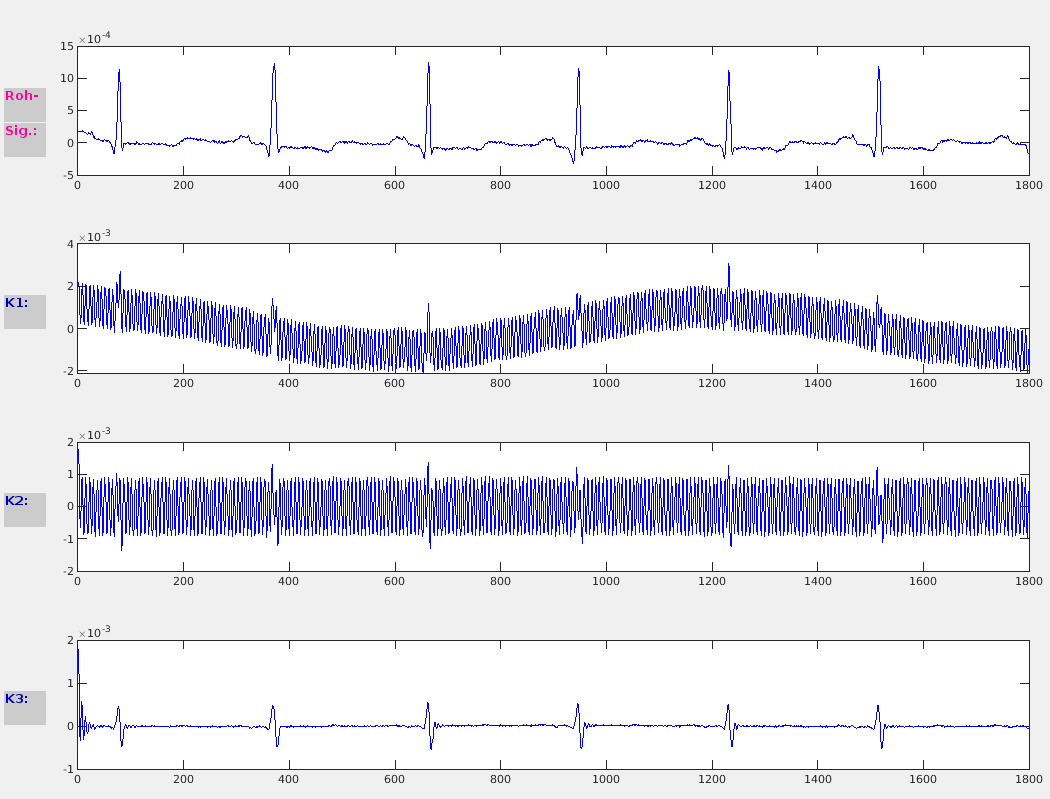
\includegraphics[width=0.9\linewidth, valign=t]{Assets/LaborBMT-15-27-08.png}
        \caption{DB100 V2}
        \label{db100v2}
    \end{minipage}%
    \begin{minipage}[t]{0.5\linewidth}
        Um das Rauschen ohne Signalverzerrung umzusetzten wird in Abbildung \ref{db100v2} von Kanal 2 auf Kanal 3 ein Notch Filter angewendet. Die Filterung von Kanal 1 auf Kanal 2 bleibt bestehen.

        Der Notch Filter entfernt das 50Hz Rauschen zuverlässig. Die Verzerrung der Form des Signals blieb jedoch bestehen.
    \end{minipage}
\end{figure}
\begin{figure}[ht]
    \begin{minipage}[t]{0.5\linewidth}
        \centering
        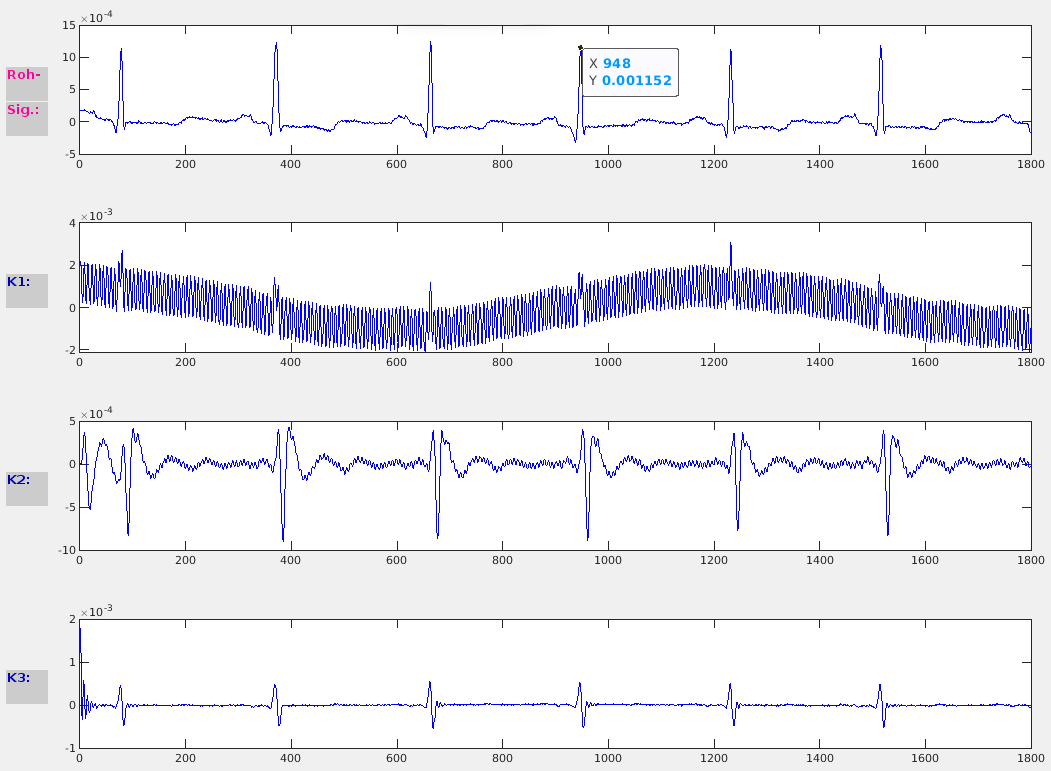
\includegraphics[width=0.9\linewidth, valign=t]{Assets/LaborBMT-15-40-04.png}
        \caption{DB100 V3}
        \label{db100v3}
    \end{minipage}%
    \begin{minipage}[t]{0.5\linewidth}
        In Abbild \ref{db100v3} ist Datenbank 100 in Kanal 2 mit einem IIR-Einseitig Bandpass 5. Ordnung des Types Butterworth mit $fo=5$ und $fu=25$ gefiltert. Kanal 3 wurde nicht verändert, das Ergebnis des letzten Notch Filters ist noch sichtbar.

        Bereits aus Kanal 2 ist ersichtlich, dass das Signal nicht die gewünschten Eigenschaften zur QRS-Erkennung haben wird. Sowohl der Amplitudengang als auch der Phasengang sind gespiegelt.
        %iir kippt den phasenfrequenzgang
    \end{minipage}
\end{figure}
\begin{figure}[ht]
    \begin{minipage}[t]{0.5\linewidth}
        \centering
        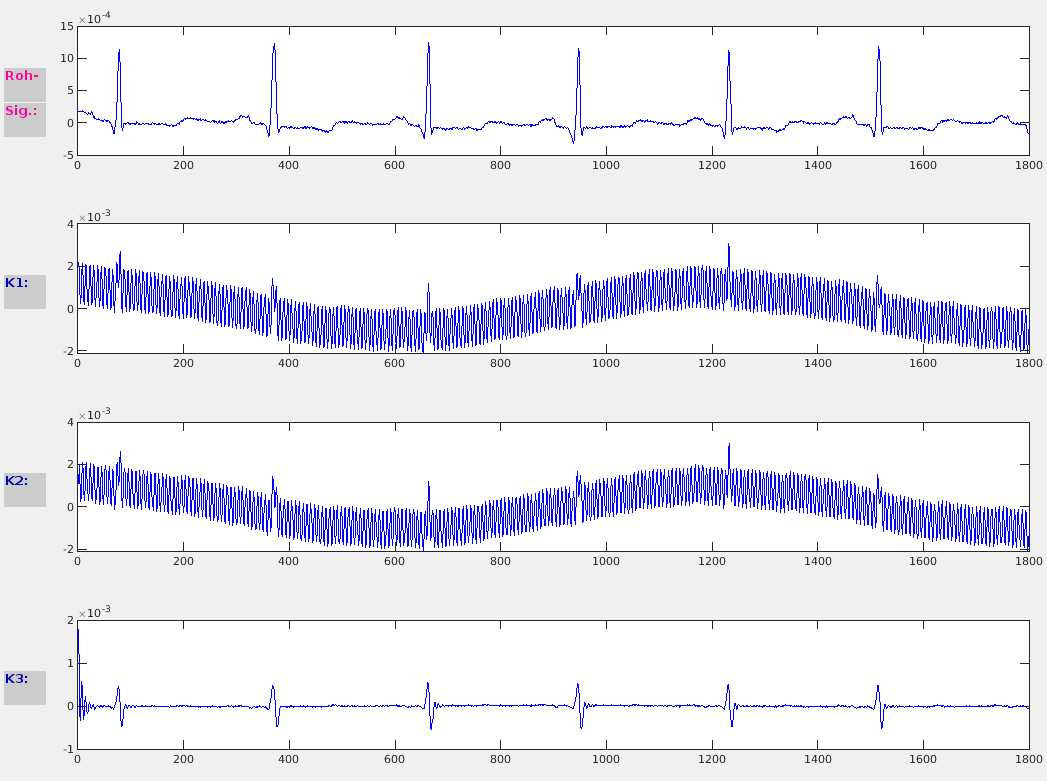
\includegraphics[width=0.9\linewidth, valign=t]{Assets/LaborBMT-15-42-26.png}
        \caption{DB100 V4}
        \label{db100v4}
    \end{minipage}%
    \begin{minipage}[t]{0.5\linewidth}
        In Abbild \ref{db100v4} ist ein Wechsel von IIR auf FIR Filtern vorgenommen worden. Aus Kanal 1 auf Kanal 2 wurde ein FIR Hochpass-Filter 1. Ordnung mit $fu=2$ angewendet. Kanal 3 ist weiterhin unverändert übernommen.

        Der Drift wurde nicht entfernt und stört weiterhin die Erkennung. Im Experiment wurde gezeigt, dass auch höhere Ordnungen dieses Filters das Signal nicht verbessern. Im nächsten Schritt wird zu einem Bandpass übergegangen.
        % fir 1. ordnung ist zu schwach, keine veränderung, keine rückführung, benötigen mehr koeffizienten -> höhere ordnung benötigt
        % FIR, hochpass, fu=2, ordnung 500
    \end{minipage}
\end{figure}
\begin{figure}[ht]
    \begin{minipage}[t]{0.5\linewidth}
        \centering
        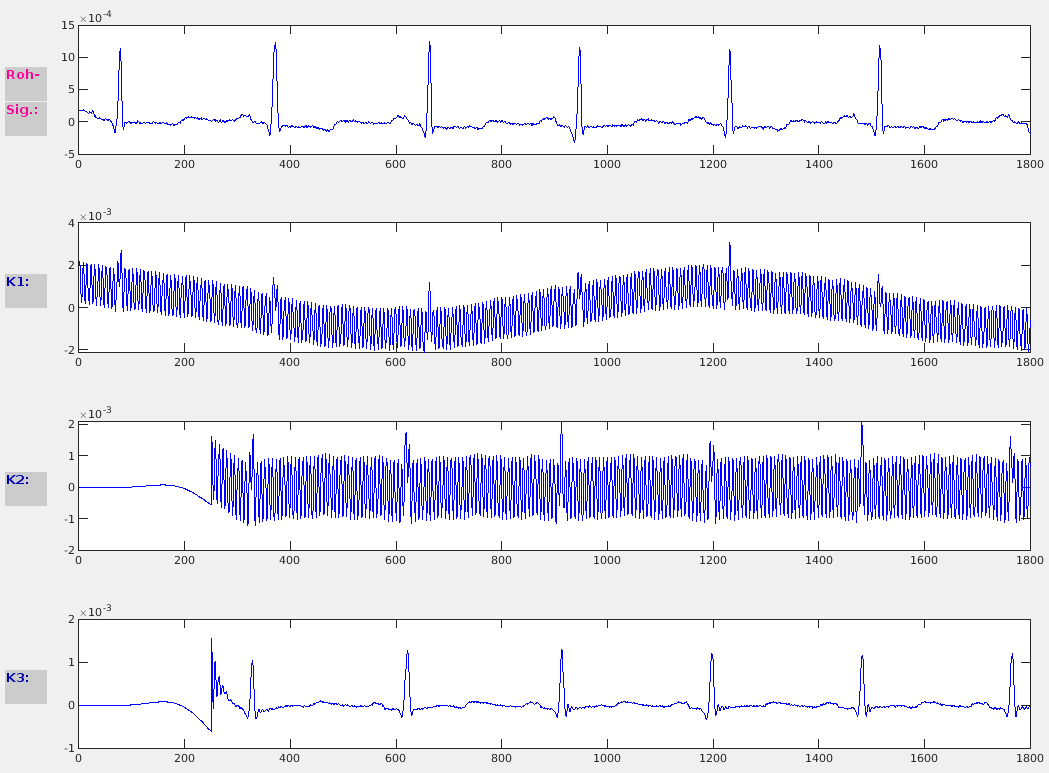
\includegraphics[width=0.9\linewidth, valign=t]{Assets/LaborBMT-15-50-45.png}
        \caption{DB100 V5}
        \label{db100v5}
    \end{minipage}%
    \begin{minipage}[t]{0.5\linewidth}
        Von Kanal 1 auf Kanal 2 wir ein einseitiger FIR-Bandpass mit $fu=2$ und $fo=30$ Hz 5. Ordnung eingesetzt.
        Von Kanal 2 auf Kanal 3 wird der Notch Filter erneut eingesetzt und in Abbildung \ref{db100v5} sichtbar.

        %warum kommt es am anfang zu niedrigen werten? hinweis blockdiagramm mit struktureinheiten
        Zu Beginn des Ausgangssignals kommt es zu niedrigen Werten. Das liegt daran, dass in jedem Arbeitsschnitt die letzten ~250ms in dem FIR Filter zur Berechnung der Filterantwort herangezogen werden.
        Zusätzlich wurde das Signal um ungefähr 250ms verzögert.

        %warum ist in k3 unten komisches gezappel?
        Bei ~250ms des Zeitverlaufs bezieht sich der Bandpass auf den ersten eingegangen Wert des K1 Signals und führt eine Nullpunktanpassung aus. Dadurch entsteht eine Signalspitze die falsch als R-Spitze erkannt werden könnte.

        Der Notch Filter entfernt das 50Hz Rauschen zuverlässig.
    \end{minipage}
\end{figure}
\begin{figure}[ht]
    \begin{minipage}[t]{0.5\linewidth}
        \centering
        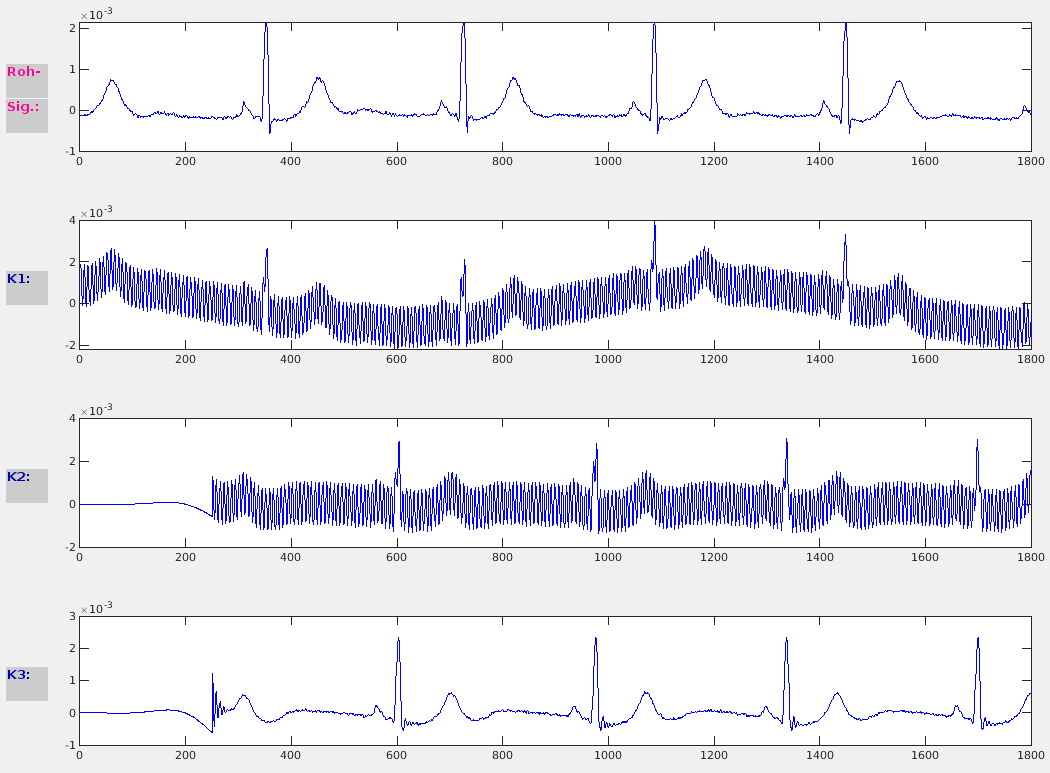
\includegraphics[width=0.9\linewidth, valign=t]{Assets/LaborBMT-15-54-32.png}
        \caption{DB106}
        \label{db106}
    \end{minipage}%
    \begin{minipage}[t]{0.5\linewidth}
        Derselbe FIR-Bandpass und Notch-Filter aus \ref{db100v5} wurde hier in Abbildung \ref{db106} verwendet und führt zu einem guten Ergebnis, aus dem die R-Spitzen klar ablesbar sind.
        %db106-> bild gleiche werte
    \end{minipage}
\end{figure}
\begin{figure}[ht]
    \begin{minipage}[t]{0.5\linewidth}
        \centering
        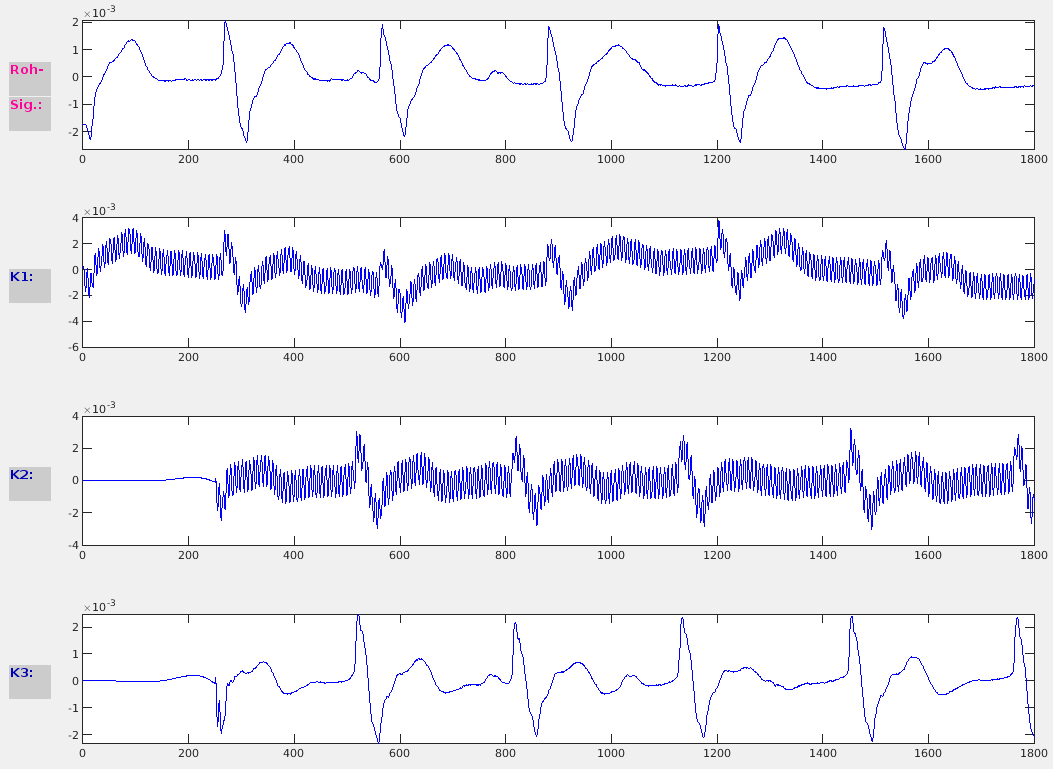
\includegraphics[width=0.9\linewidth, valign=t]{Assets/LaborBMT-15-57-50.png}
        \caption{DB108}
        \label{db108}
    \end{minipage}%
    \begin{minipage}[t]{0.5\linewidth}
        In Abbildung \ref{db108} wurde wieder der FIR-Bandpass und Notch Filter aus \ref{db100v5} verwendet. Das Ergebnis ist wieder gut und für eine Detektion nutzbar.
        %db108 -> bild, gleiche werte
        %verschiebung von k1 zu k2 mit fir
        %-> woher kommt die verschiebung, begründen, lösung?

        %welche probleme können hierbei entstehen in der analyse?
    \end{minipage}
\end{figure}


\cleardoublepage
%Lernphase= Länge der lernphase in der das signal analysisert und für die online erkennung bereit sein soll, max 250ms
%Driftkompensation, Bewegunsartefakte entfernen
%fir: finite impuls antwort
%iir: infinite impuls response
%iir könnte signal so verändern, dass pathologische fehler nicht mehr erkennbar sind, verzerrt
%- phasenverschiebung
%einseitig - online Fähig
%zweiseitig - offline fähig

Die Versuche zeigen, dass Notch-Filter eine gute Eliminierung des 50 Hz-Netz-\\rauschens erreichen. IIR- und FIR-Filter können insbesondere zur Eliminierung von niederfrequenten Störungen durch den Drift verwendet werden.
Die Realisierung mit FIR-Hochpässen ist Aufwändig, da eine hohe Filterordnung für das enge Filtergrenze vonnöten ist.

Besonders in den Abbildungen \ref{db100v5}, \ref{db106} und \ref{db108} ist auch ersichtlich, dass der FIR-Filter den Nachteil der längeren Laufzeit aufweist und damit das Signal verzögert. Dennoch liefert der FIR-Filter gute und verwertbare Ergebnisse und ist selbst durch seine Stabilität und Vorhersagbarkeit im Vergleich zum rückgekoppelten IIR-Filter von Vorteil. Aus den ersten Versuchen der Sektion \ref{EKG-Vorverarbeitung} ist dabei auch zu berücksichtigen, dass IIR-Filter das Ausgangssignal im Gegensatz zu FIR-Filtern verzerren, was Signale so verändern kann, dass pathologische Fehler nicht mehr erkennbar sind.


\subsection{QRS-Detektion mit Hilfe von MATLAB}
\texttt{Implementiere den entwickelten Algorithmus zur QRS-Detektion in die Funktion QRS\_Detektion.m}

Der Code der QRS Detektion aus den Vorbereitungsaufgaben wurde in das Programm eingefügt. Der vorgeschlagene Algorithmus verwendet einen Hochpass- und Bandpassfilter um danach mit einem aus dem Verlauf gemittelten Threshold die R-Spitzen zu erkennen.
\vspace{2cm}

\texttt{Evaluiere den QRS-Detektor anhand der EKG-Signale der MIT-Datenbank. Notiere die Detektionsquote. Wo liegen die Stärken bzw. die Schwächen des Detektors? Versuche anhand der Ergebnisse dieses ersten Detektionstests den Detektions-\\algorithmus bzw. (falls angebracht) auch die EKG-Vorverarbeitung zu optimieren! Wiederhole den Detektionstest! Inwieweit konnten die Detektionseigenschaften verbessert werden?}

\begin{figure}[ht]
    \begin{minipage}[t]{0.5\linewidth}
        \centering
        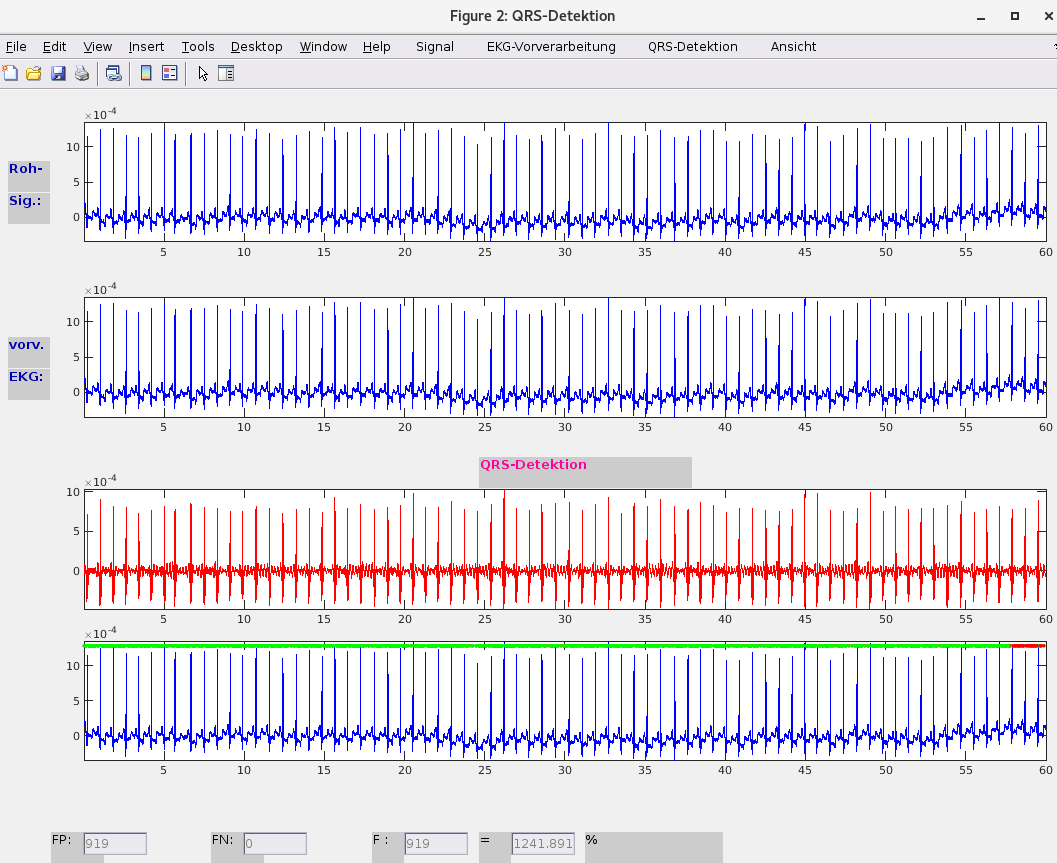
\includegraphics[width=0.9\linewidth, valign=t]{Assets/LaborBMT-16-14-54.png}
        \caption{QRS DB100}
        \label{qrsdb100}
    \end{minipage}%
    \begin{minipage}[t]{0.5\linewidth}
        Abbildung \ref{qrsdb100} zeigt den gesamten Verlauf des EKG Signals mit der QRS Detektion. Im unteren Bildteil wird die Fehlerzahl der Falsch-Positiven und Falsch-Negativen Detektionen und ein Prozentwert der Fehlerquote angezeigt.

        Der Fehler in dieser Detektion ist sehr hoch. Viele Teile des Signals wurden fälschlich als R-Zacke erkannt, was auf einen zu niedrigen Threshold hinweist. Durch den niedrigen zeitlichen Anteil der R-Spitze im Vergleich zur Dauer des Restsignals liegt der Gesamtmittelwert sehr niedrig. Der Matlab Code musste deswegen angepasst werden.

        %Db100: Bild
        % hohe Fehlerrate, zu viele Signale werden als False Positiv erkannt
        % notwendige anpassung des Matlab code; ändern von Mittelwert bilden zu Maximum Amplitude halbieren als threshold
    \end{minipage}
\end{figure}
\begin{figure}[ht]
    \begin{minipage}[t]{0.5\linewidth}
        \centering
        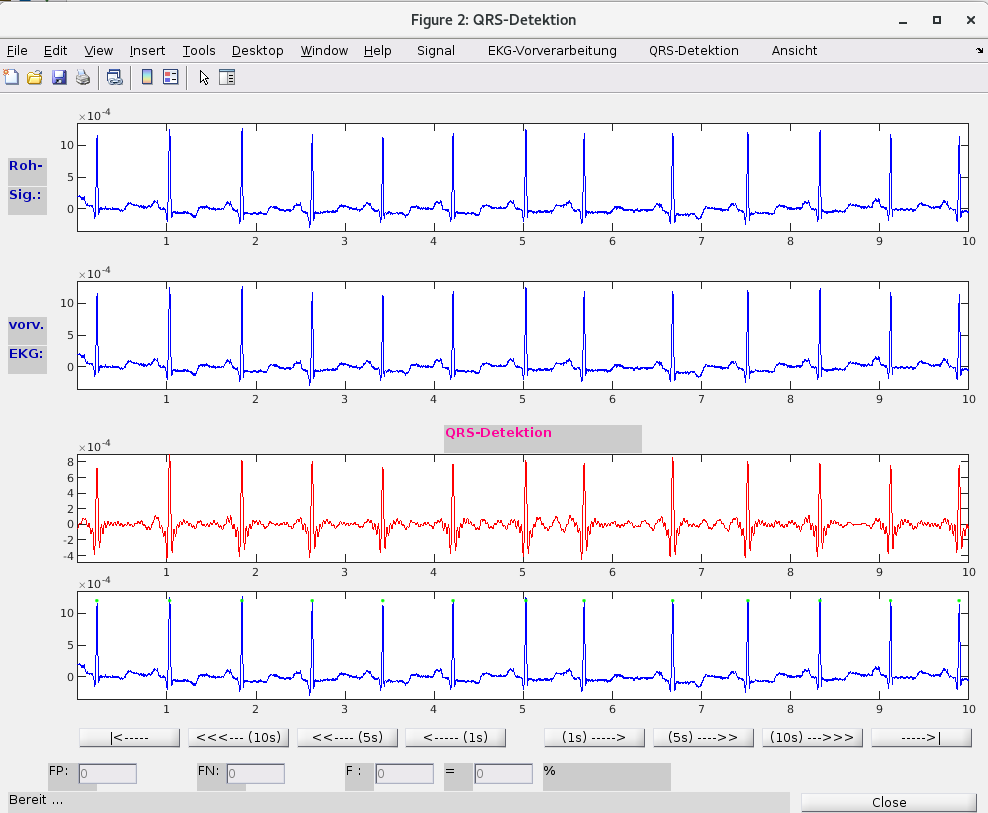
\includegraphics[width=0.9\linewidth, valign=t]{Assets/LaborBMT-16-32-42.png}
        \caption{QRS DB100 V2}
        \label{qrsdb100v2}
    \end{minipage}%
    \begin{minipage}[t]{0.5\linewidth}
        Der Treshold wird nicht mehr über den Mittelwert aller Punkte ermittelt. Stattdessen wird die maximale Amplitude bestimmt und halbiert. Dies dient dazu, nur Signale oberhalb der P-, T- und U-Wellen zu erkennen. Das sollte die Erkennung auf R-Spitzen beschränken.

        Die Erkennung für Datensatz 100 in Abbildung \ref{qrsdb100v2} ist wesentlich besser geworden im Vergleich zu Abbildung \ref{qrsdb100}.
    \end{minipage}
\end{figure}
\begin{figure}[ht]
    \begin{minipage}[t]{0.5\linewidth}
        \centering
        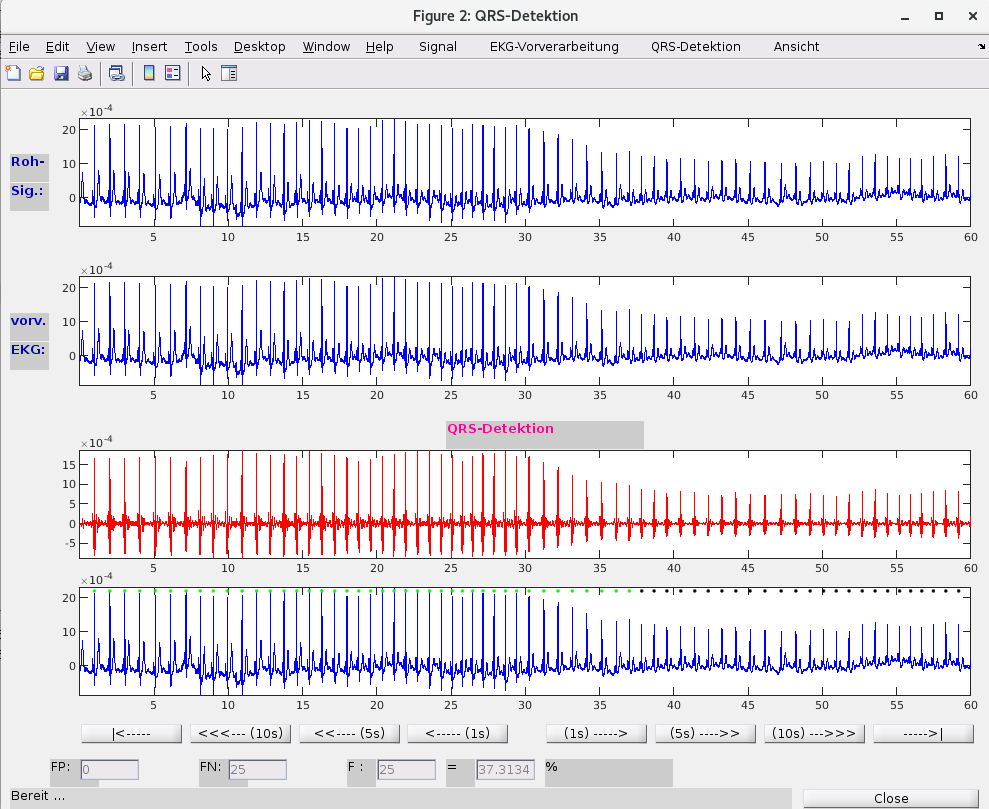
\includegraphics[width=0.9\linewidth, valign=t]{Assets/LaborBMT-16-33-27.png}
        \caption{QRS DB106}
        \label{qrsdb106}
    \end{minipage}%
    \begin{minipage}[t]{0.5\linewidth}
        In Abbild \ref{qrsdb106} sieht man die Detektion des Datensatz 106. Während die Erkennung zu Beginn gut ausfällt, fällt diese im letzten Drittel rapide herab. Das liegt an der Amplitudenänderung des Signals, an die sich der Matlab Algorithmus nicht anpasst. Stattdessen wird weiter mit dem globalen Threshold gearbeitet und R-Spitzen und diesem nicht mehr erkannt.

        Eine Verbesserung wäre durch eine aktive Schwellwertanpassung während des Verlaufs möglich (hier nicht implementiert).
        %DB106: keine anpassung des schwellwertverlaufs/tresholds an ändernde amplitude; erkennungsfehler besonders im letzten teil in dem amplitude verändert
    \end{minipage}
\end{figure}
\begin{figure}[ht]
    \begin{minipage}[t]{0.5\linewidth}
        \centering
        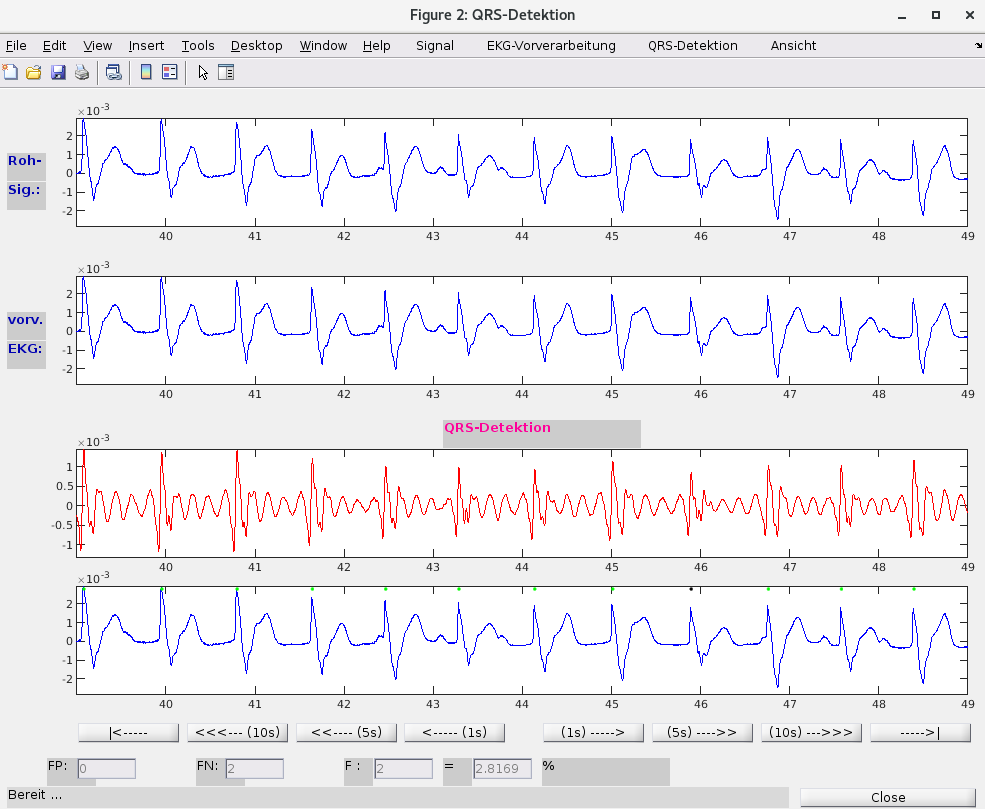
\includegraphics[width=0.9\linewidth, valign=t]{Assets/LaborBMT-16-35-29.png}
        \caption{QRS DB108}
        \label{qrsdb108}
    \end{minipage}%
    \begin{minipage}[t]{0.5\linewidth}
        Der Datensatz 108 in Abbildung \ref{qrsdb108} zeigt einen Verlauf mit erhöhter T-Welle als gewöhnlich, dies weißt auf einen Herzinfarkt im Stadium 1 hin. Da diese T-Wellen relativ hoch ausschlagen werden diese falsch Positiv erkannt.
        Der Matlab Algorithmus wurde daraufhin angepasst, indem der Schwellwert von der Hälfte der Amplitude auf das obere fünftel der Amplitude erhöht wurde. Daraufhin war die Detektion beinahe Fehlerfrei mit 2,8\% Fehlerquote, wie in der Abbildung zu erkennen. Insgesamt wurden 2 R-Spitzen nicht erkannt. Es gab keine Falsch-Positiven Detektionen.
    \end{minipage}
\end{figure}

\cleardoublepage
Der vorgeschlagene Matlab Algorithmus konnte durch Modifikation des Threshold verbessert werden aber passt sich nicht dynamisch verändernden Amplituden an.

Mögliche Adaptionen der QRS Erkennung zur verbesserten Detektion:
\begin{itemize}
    \item adaptive Schwellwertanpassung, um R-Spitzen in einer dynamisch ändernden Amplitude weiterhin korrekt zu detektieren
    \item ein minimaler und maximaler Abstand zwischen R-Spitzen um andere erhöhte Wellen von der Detektion ausschließen zu können
    \item online Fähigkeit, um die Detektion auch ohne abgeschlossene Aufnahme betreiben zu können (Bsp. EKG Monitor in der Intensivstation)
          \begin{itemize}
              \item der Threshold kann hierfür nicht aus dem Gesamtsignal ermittelt werden, stattdessen sollte ein Zeitfenster der vorhergehenden Sekunden betrachtet werden
          \end{itemize}
    \item Schwellwert stark erhöhen direkt nach Erkennen einer R-Spitze und langsam senken. Dadurch können pathologische Veränderungen der S-, T- und U-Wellen weniger Einfluss auf die Detektion nehmen. Ein exponentiell abklingender Verlauf würde sich beispielsweise anbieten, da dieser sowohl bei sehr hohem als auch bei niedrigem Puls gute Ergebnisse zu erwarten hat.
\end{itemize}

\subsection{Analyse der Herzfrequenzvariabilität}
\texttt{Analysiere die aufgezeichneten EKG-Signale während der drei Phasen RUHE, RESP und STEH. Interpretiere die Unterschiede in den Ergebnissen der einzelnen Phasen der HRV-Analyse}

Due GUI zeigt in der Herzratenvariabilität (HRV) unterschiedliche Diagramme zur Analyse auf. Das Diagramm QRS-Detektion zeigt den Verlauf des verwendeten Datensatzes in blau mit erkannten R-Spitzen in grün.
Das Diagramm ,,Herzfrequenz nach Interpolation'' darunter zeigt den zeitlichen Verlauf der Abstände zwischen zwei aufeinanderfolgenden R-Spitzen.

Das ,,HF Leistungsspektrum'' zeigt die Wahrscheinlichkeitsdichte unterschiedlicher auftretender Frequenzen über den gesamten Zeitverlauf. Durch Ausprägung markanter Formen können pathologische Veränderungen erkannt werden.

Das Scatter- und Phasendiagramm sind weitere Darstellungsformen für die Variabilität. Je weiter verstreut die Punkte, welche die aufeinanderfolgenden Abstände der R-Spitzen darstellen, liegen desto größer ist die HRV. Im gesunden Fall erwarten wir eine elliptische Form des Streudiagramms; andere Ausprägungen können beispielsweise auf Herzrythmusstörungen hinweisen.

Das Histogramm ist das letzte Diagramm der GUI. Die gemessenen R-Spitzen-Abstände werden in feste Zeitbereiche gegliedert und als Balken über die prozentuale Häufigkeit des bestimmten Wertes dargestellt. Die Anzahl der Balken ist abhängig von der Variabilität des Probanden. Im gesunden Fall erwarten wir grob die Form einer Gaußkurve. Andere Formen können auf pathologische Veränderungen oder weitere äußere Einflüsse während der Messung (Bsp. starke Atmung) hinweisen.

\begin{figure}[ht]
    \begin{minipage}[t]{0.5\linewidth}
        \centering
        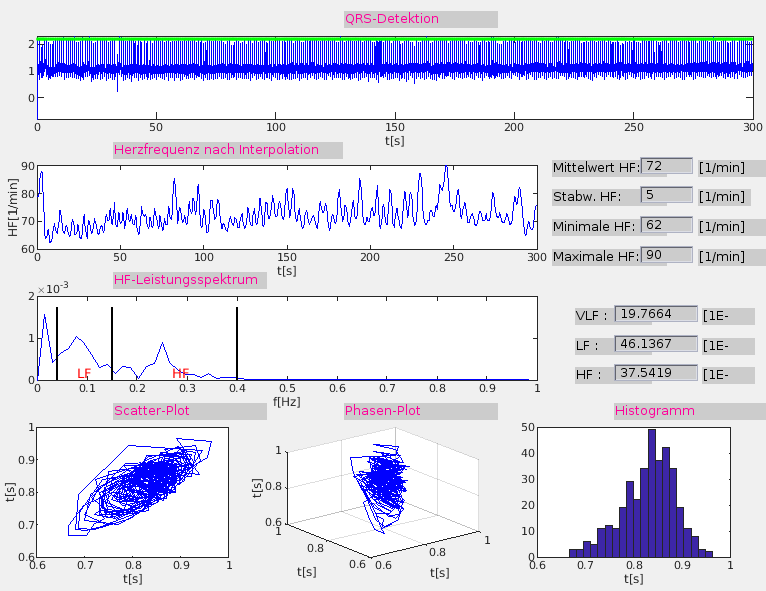
\includegraphics[width=0.9\linewidth, valign=t]{Assets/LaborBMT-16-59-32.png}
        \caption{Phase RUHE}
        \label{phaseruhe}
    \end{minipage}%
    \begin{minipage}[t]{0.5\linewidth}
        In der Ruhephase sitzt und atmet der Proband normal.

        Das Diagramm nach Interpolation zeigt kleine Amplitudenänderungen bei großer Signalanzahl.

        Im HF-Leistungsspektrum sind drei markante Spitzen ersichtlich. Diese entsprechen den in der Praktikumsanleitung (S.24) beschriebenen thermoregulatorischen Vorgängen im sehr niederfrequenten (VLF) Bereich, Blutdruckwellen III. Ordnung im niederfrequenten (LF) Bereich und Einflüsse der Atmung im hochfrequenten (HF) Bereich.

        Der Scatter-Plot und Phasen-Plot zeigen eine gering gestreute Anordnung und eine etwa elliptische Form.

        Im Histogramm erkennt man die erwartete gaußsche Glockenkurvenform.

        Die Diagramme zeigen alle die erwarteten und in der Literatur beschriebenen Eigenschaften und weisen auf einen gesunden Probanden hin.

        %atmiung/atemfrequenz kann einfluss haben , hf
        %blutdruck hat einfluss, besonders im stehen, lf
    \end{minipage}
\end{figure}
\begin{figure}[ht]
    \begin{minipage}[t]{0.5\linewidth}
        \centering
        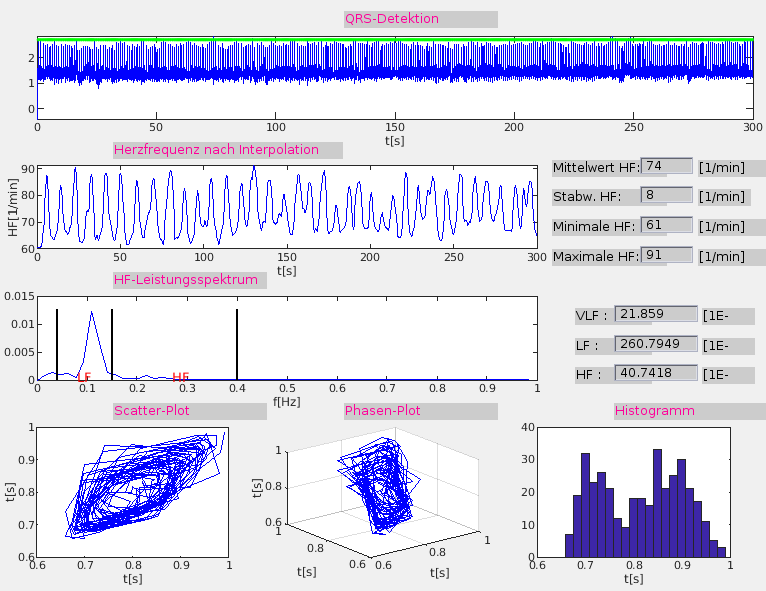
\includegraphics[width=0.9\linewidth, valign=t]{Assets/LaborBMT-17-00-21.png}
        \caption{Phase RESP}
        \label{phaseresp}
    \end{minipage}%
    \begin{minipage}[t]{0.5\linewidth}
        In der Respirationsphase sitzt der Proband und atmet langsam tief ein und tief aus.

        Das Diagramm nach Interpolation zeigt große Amplitudenänderungen. Im Vergleich zum vorhergehenden Datensatz bleibt die Amplitudendifferenz im zeitlichen Verlauf sehr konstant.

        Im HF-Leistungsspektrum ist eine markante Spitzen im niederfrequenten (LF) Bereich zu sehen. Diese entspricht der erwarteten Ausprägung durch starke Atmung. Jedoch aufgrund der langsamen Atmung in den niederfrequenten (LF) Bereich verschoben.

        Der Scatter-Plot und Phasen-Plot zeigen eine elliptische Ausprägung bei breitere Streuung der Datenpunkte.

        Im Histogramm erkennt man zwei ausprägungen der erwarteten Gaußkurven, die einander teilweise überlagern; entsprechend der Ein- und Ausatemphasen.

    \end{minipage}
\end{figure}
\begin{figure}[ht]
    \begin{minipage}[t]{0.5\linewidth}
        \centering
        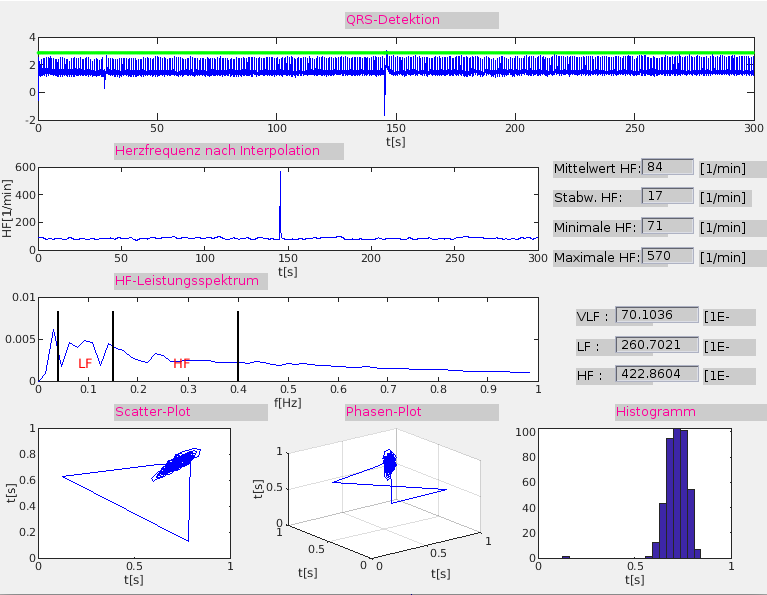
\includegraphics[width=0.9\linewidth, valign=t]{Assets/LaborBMT-17-09-35.png}
        \caption{Phase STEH}
        \label{phasesteh}
    \end{minipage}%
    \begin{minipage}[t]{0.5\linewidth}
        In der Stehphase steht der Proband und atmet normal.

        Aus der QRS-Detektion und den Scatter- und Phasenplot ist ein, wahrscheinlich aus einem Bewegungsartefakt resultierender, Ausreißer ersichtlich. Dieser muss hier einmalig manuell im Code behoben werden, indem der Datenpunkt genullt wird. Die korrigierte Detektion ist in Abbildung \ref{phasesteh2} sichtbar und zeigt deutlich, wie ein einzelner Ausreißer die Auswertung verfälschen kann.

        %ausreißer an position 204 wurde im matlab code genullt
        %diagramme dadurch korrigiert
    \end{minipage}
\end{figure}
\begin{figure}[ht]
    \begin{minipage}[t]{0.5\linewidth}
        \centering
        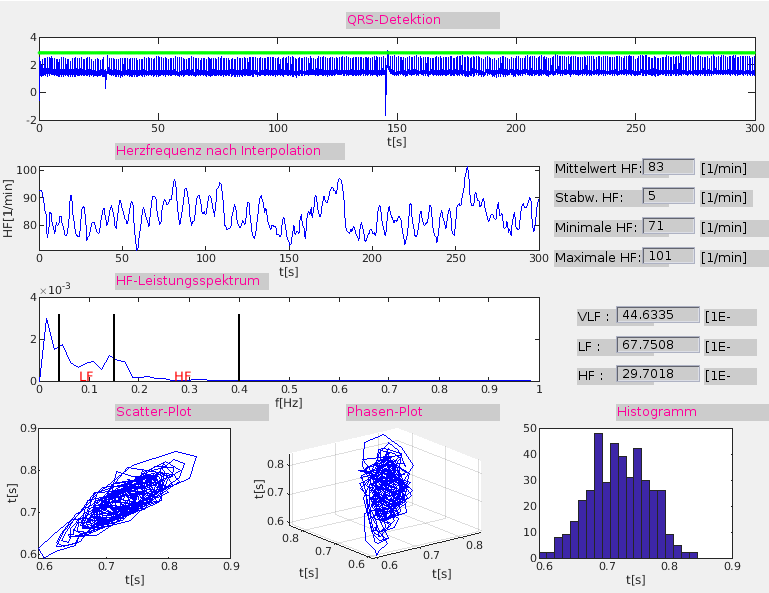
\includegraphics[width=0.9\linewidth, valign=t]{Assets/LaborBMT-17-25-19.png}
        \caption{Phase STEH Korrigiert}
        \label{phasesteh2}
    \end{minipage}%
    \begin{minipage}[t]{0.5\linewidth}

        Das Diagramm nach Interpolation zeigt eine hohe Variabilität im Zeitverlauf.

        Im HF-Leistungsspektrum sind eine Spitze im sehr niederfrequenten (VLF) Bereich erkennbar, sowie eine breite Signaldichte im niederfrequenten (LF) Bereich. Der hochfrequente (HF) Bereich ist weitestgehend frei von Signalen. Im Vergleich zur Ruhephase sehen wir einen höheren Einfluss der sehr niederfrequenten Anteile (z.B. Blutdruck, thermoregulatorische Vorgänge) auf das Gesamtspektrum.

        Der Scatter-Plot und Phasen-Plot zeigen eine in die Länge gezogene Ellipse mit hoher Dichte.

        Im Histogramm erkennt man eine Gaußkurve mit wenigen Spitzen in der Mitte. Im Vergleich zur Ruhephase ist die Gaußkurve nach links verschoben, was von der höheren Herzfrequenz herrührt.

        %frequenz: atmung bildet sich ab,
        %bewegung
        %ausreißer,
        %woher komtm die energie, bltudruck
    \end{minipage}
\end{figure}
\cleardoublepage

\texttt{Vergleiche die HRV-Ergebnisse des Praktikumsprobanden mit den Ergebnissen eines Polyneuropathie-Patienten.}

Polyneuropathie ist eine Gruppe von Erkrankungen, bei der mehrere periphere Nerven geschädigt sind. Bekannte Symptome sind unter anderem Muskelschwäche, Muskelkrämpfe und Lähmungen.

Zu beachten ist die verkürzte Laufzeit des Datensatzes in \ref{zwickau} von ~180 Sekunden im Vergleich zu den Standard 300 Sekunden Aufnahmen der Datensätze \ref{phaseruhe}, \ref{phaseresp} und \ref{phasesteh2}. Außerdem ist zu beachten, dass die Amplituden der QRS-Detektion sich sehr stark von den Erwartungen am gesunden Probanden unterscheiden, ob es sich hierbei um eine andere Größenordnung als mV handelt ist aus dem Diagramm nicht ersichtlich.

\begin{figure}[ht]
    \begin{minipage}[t]{0.5\linewidth}
        \centering
        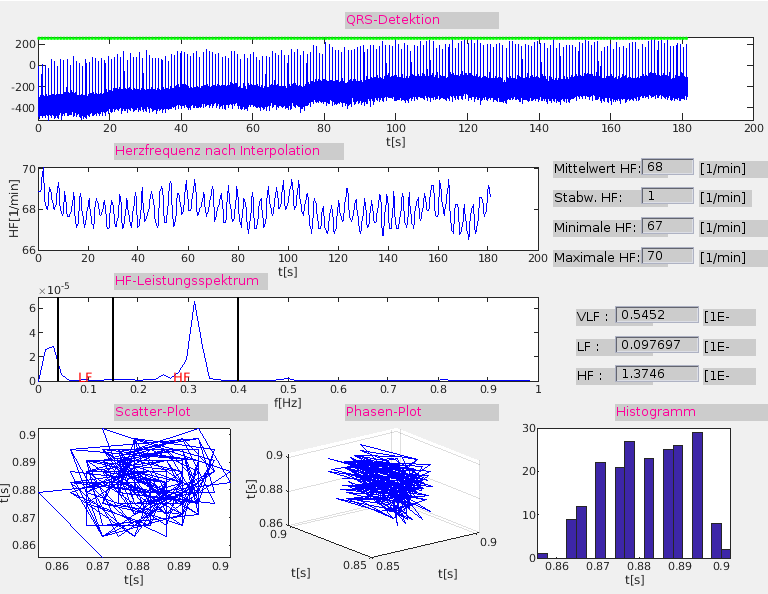
\includegraphics[width=0.9\linewidth, valign=t]{Assets/LaborBMT-17-30-09.png}
        \caption{Polyneuropathie}
        \label{zwickau}
    \end{minipage}%
    \begin{minipage}[t]{0.5\linewidth}
        Das Diagramm nach Interpolation zeigt eine gleichmäßige Herzrate mit geringer Variabilität.

        Im HF-Leistungsspektrum sind eine Spitze im sehr niederfrequenten (VLF) Bereich und eine im hochfrequenten (HF) Bereich abzulesen. Dies unterscheidet sich deutlich von gesunden Probanden.

        Im Phasen-Plot erkennt man eine geringe Verteilung, die auf eine geringe Variabilität zurückzuführen ist. Die Form des Scatter- und Phasen-Plot weißt zudem keine Ellipse auf was auf eine mögliche Herzrythmusstörungen hindeutet.

        Im Histogramm ist keine Gauß Verteilung sichtbar. Deutlich erkennbar sind hier vorallem Lücken. Auch dies weißt auf eine Herzrythmusstörung hin.

        %polyneurapathie
        %woher kommen Auswirkungen
        %woran erkennt man das
        %histogram
        %physiologische und phatologische unterschiede und woran erkennt man das?
    \end{minipage}
\end{figure}

Ein Vergleich mit den HRV-Analysen in Abbildungen \ref{phaseruhe}, \ref{phaseresp} und \ref{phasesteh2} zeit deutlich erkennbare Unterschiede auf, die für eine Diagnose des Probanden genutzt werden können. 
Alle Diagramme in Abbildung \ref{zwickau}zeigen eine sehr kleine Verteilung und Herzfrequenzvariabilität. Die Herzrate ist sehr gleichmäßig. Über die Verteilung im Phasen-Diagramm sind sehr enge R-Spitzen-Abstände zu sehen. Diese deuten ohne Vorwissen der Erkrankung auf ein Problem mit dem Nervensystem hin. Die Ausformung des Histogramms und Scatter-Diagramms weisen zusätzlich auf eine mögliche Herzrythmusstörungen hin. 
Nach den Spitzen des HF-Leistungsspektrums wurde das EKG vermutlich während der Respirationsphase aufgenommen.

\newpage
\section{Quellen}
\begin{itemize}
    \item Prof. Dr.-Ing. habil. Peter Husar, Vorlesung ,,Grundlagen der Biosignalverarbeitung'', TU Ilmenau, 2021
    \item M.Sc. Marc-Patrick Heppner, Praktikumsanleitung ,,EKG Signalanalyse'', TU Ilmenau, 2021
    \item Univ.-Prof. Dr.-Ing. Martin Haardt, Vorlesung ,,Signale und Systeme 1'', TU Ilmenau, 2019 
    \item \href{https://eleceng.dit.ie/dorran/matlab/resources/Matlab%20Signal%20Processing%20Examples.pdf}{eleceng.dit.ie}, Matlab Beispiele, Abgerufen 11.01.2021
    \item \href{https://biomedicalsignalandimage.blogspot.com/2016/02/matlab-code-to-plot-ecg-signal.html}{biomedicalsignalandimage.blogspot.com}, Matlab EKG Beispiel, Abgerufen 11.01.2021
    \item \href{https://github.com/Aburas98/MATLAB/}{GitHub.com/Aburas98}, Matlab EKG Beispiele, Abgerufen 04.01.2021
    \item \href{https://www.section.io/engineering-education/electrocardiograms-qrs-peak-and-heart-rate-detection-using-dwt-in-matlab/}{section.io}, QRS Detektion Beispiel, Abgerufen 11.01.2021
    \item \href{https://de.mathworks.com/help/dsp/ug/real-time-ecg-qrs-detection.html}{Mathworks.com}, EKG Analyse, Abgerufen 04.01.2021
    \item \href{https://www.netdoktor.de/krankheiten/polyneuropathie/}{Netdoktor.de}, Polyneuropathie, Abgerufen 25.01.2021
    \item Karl Dirk Kammeyer: Digitale Signalverarbeitung. 6. Auflage. Teubner, 2006, ISBN 3-8351-0072-6
\end{itemize}

\listoffigures

\newpage
\section{Anhang: Überarbeiteter Code}
\begin{lstlisting}[basicstyle=\scriptsize, language=matlab]
function [R_Positionen, Entscheidungssignal, Schwellwertverlauf, Lernphase] 
= QRS_Detektion (EKG_Signal, fa);
    size = length(EKG_Signal); % Laenge des Signals
    % fourier transformation
    signal = fft(EKG_Signal);
    % entfernen niedriger freqzenzen anhand Laenge und Rate
    signal(1 : round(size*5/fa))=0;
    signal(end - round(size*5/fa) : end)=0;
    % inverse fourier transformation
    signal=real(ifft(signal));
    
    % bandpass fuer 5 bis 30 hz
    signal=bandpass(signal, [5 30], fa);
    
    % skalierung des Signals auf skala 1-10
    filtersignal=signal/(max(signal)/10);
    % entfernen aller peaks unterhalb des thresholds 10/2=5
    for data = 1:1:length(filtersignal)
        if filtersignal(data) < 5
            filtersignal(data) = 0;
        else
            filtersignal(data)=1;
        end
    end
    % finde alle uebrigen peaks, die ueber dem threshold lagen
    positions=find(filtersignal);
    % abstand der ersten beiden peaks
    distance=positions(2)-positions(1);
    % setzte den abstand auf das minimum zweier peaks in der reihe aller uebrigen peaks
    for data=1:1:length(positions)-1
        if positions(data+1)-positions(data)<distance
            distance=positions(data+1)-positions(data);
        end
    end
    
    % Mittel der Signalamplitude als Threshold
    avg = (max(signal)/5)*4; 
    
    % Absolute Peaks innerhalb des Zeitfensters finden
    [RPeaks, positions] = findpeaks(signal, 'MinPeakHeight', avg, 
                'MinPeakDistance', distance, "MaxPeakWidth", 250);
    % positions[242] = 0; % optional zum entfernen von Ausschlaegen
    R_Positionen = positions;
    Entscheidungssignal = signal;
    Schwellwertverlauf = signal; % nicht verwendet
    Lernphase = 0; % nicht verwendet
end
\end{lstlisting}
\end{document}